% Copyright 2020 by Robert Hildebrand
%This work is licensed under a
%Creative Commons Attribution-ShareAlike 4.0 International License (CC BY-SA 4.0)
%See http://creativecommons.org/licenses/by-sa/4.0/

%\documentclass[../open-optimization/open-optimization.tex]{subfiles}
%
%\begin{document}

\chapter{Algorithms to Solve Integer Programs}
\todoChapter{ 50\% complete. Goal 80\% completion date: September 20\\
Notes: }
\label{sec:IP-algorithms}

\begin{outcome}
\begin{enumerate}
\item Understand misconceptions in difficulty of integer programs
\item Learn basic concepts of algorithms used in solvers
\item Practice these basic concepts at an elementary level
\item Apply these concepts to understanding output from a solver
\end{enumerate}
\end{outcome}

In this section, we seek to understand some of the fundamental approaches used for solving integer programs.   These tools have been developed the past 70 years.  As  such, advanced solvers today are incredibly complicated and have many possible settings to hope to solve your problem more effiently.  Unfortunately, there is no single approach that is best for all different problems.

\includefigurestatic[GUROBI Performance on a set of problems while varying different  possible settings.  This plot show the wild variablity of performance of different approaches.  Thus, it is very unclear which is the ``best" method. Furthermore, this plot can look quite different depending on the problem set one is working with.   Altough we will not emphasize determining optimal settings in this text, we want to make clear that the techniques used in solvers are quite complicated and are tuned very carefully.  We will study some elementary versions of techniques used in these solvers.][width=0.90\linewidth][h]{gurobi_performance}

Although there are many tricks used to imrove the solve time, there are thee core elements to solving an integer program: \emph{Presolve}, \emph{Primal techniques}, \emph{Cutting Planes}, and \emph{Branch and Bound}.   

\paragraph{Presolve} contains many tricks to elimate variables, reduce the problem size, and make format the problem into something that might be easier to solve.  We will not focus on this aspect of solving integer programs.

\paragraph{Primal techniques} use a variety of approaches to try to find feasible solutions.  These feasible solutions are extemely helpful in conjunction with branch and bound.

\paragraph{Cutting planes} are ways to improve the description by adding additional inequalities.  There are many ways to derive cutting planes.  We will learn just a couple to get an idea of how these work.  

\paragraph{Brach and bound} is a method to decompose the problem into smaller subproblems and also to certify optimality (or at least provide a bound to how close to optimal a solution is) by removing sets of subproblems that can be argued to be suboptimal.   We will look at an elementary branch and bound approach.  \underline{Understanding this technique is key to explaining the ouput of an integer programming solver.}


We will being this chapter with a comparison of solving the linear programming relaxation comparted to solving an integer program.  We will then use this understanding as fundamental to both the techniques of cutting planes and branch and bound.
We will end this section with an example of output from GUROBI and explain how to interpret this information.

\section{Foundational Principle - LP is a relaxation for IP}
\begin{outcome}
This section decribes the foundational princple about relaxations that will be used in our main algorithmic techniques.
\end{outcome}

Recall that the linear relaxation of an integer program is the linear programming problem after removing the integrality constraints
$$
\begin{array}{rlclr}
\text{ Integer Program:} & & & \text{Linear Relaxation:}\\
\max \ & z_{IP} = c^\top x & \hspace{3cm} & & \max \  z_{LP} = c^\top x \\
& Ax \leq b & & & Ax \leq b\\
& \tred{x \in \Z^n} & & & \tblue{x \in \R^n}
\end{array}
$$

\begin{theorem}{LP Bounds}{}
It always holds that 
\begin{equation}
z^*_{IP} \leq z^*_{LP}.
\end{equation}
Furthermore, if $x^*_{LP}$ is integral (feasible for the integer program), then 
\begin{equation}
x^*_{LP} = x^*_{IP} \ \ \text{ and } z^*_{LP} = z^*_{IP}.
\end{equation}
\end{theorem}

\begin{example}{}{}

%%second column
%\begin{minipage}[t]{0.1\textwidth}
%\includegraphics[scale = 0.3]{LP-equals-IP.png}
%\end{minipage}
%
%Here is some text.\\
% first column
\begin{minipage}[t]{0.5\textwidth}
Consider the problem 
\begin{align*}
\max z = & 3x_1 + 2x_1\\
& 2x_1 + x_2 \leq 6\\
& x_1, x_2 \geq 0; x_1, x_2 \text{ integer}
\end{align*}
\end{minipage}
%
%second column
\begin{minipage}[t]{0.4\textwidth}
%This is the graph
\end{minipage}
\end{example}


%  \includegraphics[width=2cm,height=2cm]{LP-equals-IP.png}\fbox{\LARGE J}
  
  
  \subsection{Rounding LP Solution can be bad!}

  Consider the two variable knapsack problem
  \begin{align}
  \max   3x_1 + 100 x_2\\
              x_1  + 100 x_2 \leq 100\\
              x_i \in \{0,1\} \text{ for } i=1,2.
  \end{align}
  
  Then $x^*_{LP} = (1, 0.99)$ and $z^*_{LP} = 1\cdot 3 + 0.99\cdot 100 = 3 + 99 = 102.$
  
  But $x^*_{IP} = (0,1)$ with $z^*_{IP} = 0\cdot 3 + 1 \cdot 100 = 100$.
  
  Suppose that we rounded the LP solution.  
  
  $x^*_{LP-Rounded-Down} = (1,0)$.  Then $z^*_{LP-Rounded-Down} = 1\cdot 3 = 3$.  Which is a terrible solution!
  
  
  How can we avoid this issue?  We will use two main techniques - (1) decomposing the problem via \emph{Branch and Bound} and (2) improve the LP relaxation via cutting planes.
    
  \subsection{Rounding LP solution can be infeasible!}
  Now only could it produce a poor solution, it is not always clear how to round to a feasible solution.  
    Consider the two variable knapsack problem
  \begin{align}
  \min   x_1 + 200 x_2\\
              x_1  + 100 x_2 \geq 100\\
              x_i \in \{0,1\} \text{ for } i=1,2.
  \end{align}
  Again, we return  $x^*_{LP} = (1, 0.99)$.  But in this case, rounding down to $(1,0)$ is not feasible!
  
  In $n$-dimensions, there are potentially $2^n$ integer points to round to, making rounding very complicated in some cases.
 



\section{Branch and Bound}
\subsection{Binary Integer Programming}
Our goal is to decompose the problem until one of three things happens:
\begin{enumerate}
\item We find an \textbf{integer} point in a subproblem,
\item We prove that a sub problem is \textbf{suboptimal},
\item We prove that a subproblem is \textbf{infeasible}.
\end{enumerate}
Throughout the decomposition process, we will store Lower Bounds.  These bounds are created by finding feasible integer solutions.  Using these lower bounds, we can prove that other branches are suboptimal.


Here is the full algorithm.  We will look at an example next.
\begin{algorithm}[H]
\caption{Branch and Bound for Binary Integer Programming}\label{alg:branch-and-bound-bip}
\begin{algorithmic}[1]
    \Require Binary Integer Linear Problem with max objective
    \Ensure Exact Optimal Solution $x^*$
    \State Set $LB = - \infty$.
    \State Solve LP relaxation. 
    \If{$x^*$ is binary integer}
        \State Stop!
    \Else
        \State Choose fractional entry $x_i^*$.
        \State Branch onto subproblems:
        \Statex \hspace{2em} (i) $x_i = 0$
        \Statex \hspace{2em} (ii) $x_i = 1$
    \EndIf
    \State Solve LP relaxation of any subproblem.
    \If{LP relaxation is infeasible}
        \State Prune this node as \textbf{"Infeasible"}
    \ElsIf{$z^* < LB$}
        \State Prune this node as \textbf{"Suboptimal"}
    \ElsIf{$x^*$ is binary integer}
        \State Prune this node as \textbf{"Binary Integer"}
        \State Update $LB = \max(LB, z^*)$.
    \Else
        \State Choose fractional entry $x_i^*$.
        \State Branch onto subproblems:
        \Statex \hspace{2em} (i) $x_i = 0$
        \Statex \hspace{2em} (ii) $x_i = 1$
        \State Return to step 2 until all subproblems are pruned.
    \EndIf
    \State Return best binary integer solution found.
\end{algorithmic}
\end{algorithm}


Let's look at a nice example.  This is the smallest example that exhibits all the interesting behavior of branch and bound.  Typically these branch and bound trees are much much much bigger.

We will use the result from Subsection~\ref{subsection:fractional-knapsack} that demonstrates that in the single inequality case, the solution to the LP can be easy to write down.

%\textbf{Example: Binary Knapsack}
\begin{example}{Binary Knapsack Example}{}
Solve the following problem with branch and bound.
\begin{align*}
\max\ \ \   z&=11x_1+15x_2+6x_3+2x_4 + x_5\\
\text{Subject to:} \ \ \ 	 &5x_1+7x_2+4x_3+3x_4 + 15x_5\leq15\\
		&x_i  \text{  binary},i=1,\dots,5
\end{align*}

% Branch and bound tree for maximize knapsack
\tikzset{
  S/.style = {draw, rectangle, rounded corners=0.1cm, minimum size = 8mm,  top color=blue!10, bottom color=blue!10},% top color=white, bottom color=blue!20},
}
     \begin{tikzpicture}[-,thick]
\node[S,sibling distance=5cm, level distance=1.3cm, align=left, label={[blue]left:$t = 1$}, label = {above:\textbf{Root Node}}] 
	{$x^* = (1,1,0.75,0,0) $\\ $z^* = 30.5$\\ $ LB = -\infty$} 
	[sibling distance=7cm, level distance=2.8cm,align=left]
	%
     	child {node[S, label={[blue]left:$t = 2$}, label = {[red]below: \rule{3cm}{0.8pt} \\ \centering Integer}] 
     		{$x^* = (1,1,0,1,0) $\\$z^* = 28$\\$ LB = 28$}
		[sibling distance=2.5cm, level distance=2.8cm,align=left]
   		edge from parent node[left] {$x_3 = 0$}
   }
     child {node[S, label={[blue]right:$t =3$}] 
     		{$x^* = (1,0.857,1,0,0) $\\$z^* = 29.857$\\$ LB = 28$}
		[sibling distance=5cm, level distance=2.8cm,align=left]
		%
     		child {node[S, label={[blue]left:$t = 4$}, label = {[red]below: \rule{3cm}{0.8pt} \\ \centering Suboptimal}] {$x^* = (1,0,1,1,0.2)$\\$z^* = 19.2$\\$ LB = 28$}
     			edge from parent node[left] {$x_2 = 0$}}
     		child {node[S, label={[blue]right:$t =5$}] {$x^* = (0.8,1,1,0,0)$\\$z^* = 29.8$\\$ LB = 28$}[sibling distance=5cm, level distance=2.8cm,align=left]
			child {node[S, label={[blue]left:$t =6$}, , label = {[red]below: \rule{3cm}{0.8pt} \\ \centering Suboptimal}] {$x^* = (0,1,1,1,0.067)$\\$z^* = 23.067$\\$ LB = 28$}[sibling distance=5cm, level distance=2.8cm,align=left]
				edge from parent node[left] {$x_1 = 0$}
				}
			child {node[S, label={[blue]right:$t =7$}, label = {[red]below: \rule{3cm}{0.8pt} \\ \centering Infeasible}] {\\ Infeasible \hspace{3cm} \\ }[sibling distance=5cm, level distance=2.8cm,align=left]
				edge from parent node[right] {$x_1 = 1$}
				}
     			edge from parent node[right] {$x_2 = 1$}
			}
   		edge from parent node[right] {$x_3 = 1$}
   };

     \end{tikzpicture}


An optimal solution is concluded to be $x^* = (1,1,0,1,0)$ with objective value $z^* = 28$.

\end{example}
\subsection{Branch and bound on general integer variables}

We can apply this concept of branch and bound thinking about general integer variables.  Instead of branching to specific values, we restrict to upper and lower bounds on a variable.  This cuts the feasible region of a problem (or sub problem) into two smaller regions.  All of the same concepts apply here.

\begin{algorithm}[H]
\caption{Branch and Bound - Maximization}\label{alg:branch-and-bound-max}
\begin{algorithmic}[1]
    \Require Integer Linear Problem with max objective
    \Ensure Exact Optimal Solution $x^*$
    \State Set $LB = - \infty$.
    \State Solve LP relaxation. 
    \If{$x^*$ is integer}
        \State Stop!
    \Else
        \State Choose fractional entry $x_i^*$.
        \State Branch onto subproblems:
        \Statex \hspace{2em} (i) $x_i \leq \lfloor x^*_i \rfloor$
        \Statex \hspace{2em} (ii) $x_i \geq \lceil x^*_i \rceil$
    \EndIf
    \State Solve LP relaxation of any subproblem.
    \If{LP relaxation is infeasible}
        \State Prune this node as \textbf{"Infeasible"}
    \ElsIf{$z^* < LB$}
        \State Prune this node as \textbf{"Suboptimal"}
    \ElsIf{$x^*$ is integer}
        \State Prune this node as \textbf{"Integer"}
        \State Update $LB = \max(LB, z^*)$.
    \Else
        \State Choose fractional entry $x_i^*$.
        \State Branch onto subproblems:
        \Statex \hspace{2em} (i) $x_i \leq \lfloor x^*_i \rfloor$
        \Statex \hspace{2em} (ii) $x_i \geq \lceil x^*_i \rceil$
        \State Return to step 2 until all subproblems are pruned.
    \EndIf
    \State Return best integer solution found.
\end{algorithmic}
\end{algorithm}

%\begin{algorithm}[H]
%\algorithmicrequire{Integer Linear Problem with max objective}\\
%\algorithmicensure{Exact Optimal Solution $x^*$}
%\caption{Branch and Bound - Maximization}\label{alg:branch-and-bound-max}
%\begin{algorithmic}[1]
%	\State Set $LB = - \infty$.
% 	\State Solve LP relaxation. 
%	\begin{algsubstates}
%        		\State If $x^*$ is integer, stop!
%        		\State Otherwise, choose fractional entry $x_i^*$ and branch onto subproblems:
%		(i) $x_i \leq \lfloor x^*_i \rfloor$ and 
%		(ii) $x_i \geq \lceil x^*_i \rceil$.    
%	   \end{algsubstates}
%	\State Solve LP relaxation of any subproblem.
%		\begin{algsubstates}
%		\State If LP relaxation is infeasible, prune this node as \textbf{"Infeasible"}
%        		\State If $z^* < LB$, prune this node as \textbf{"Suboptimal"}
%		\State $x^*$ is integer, prune this nodes as \textbf{"Integer"} and update $LB = \max(LB, z^*)$.
%		\State Otherwise, choose fractional entry $x_i^*$ and branch onto subproblems:  (i) $x_i \leq \lfloor x^*_i \rfloor$ and (ii) $x_i \geq \lceil x^*_i \rceil$.     Return to step 2 until all subproblems are pruned.
%      \end{algsubstates}
%      \State Return best integer solution found.
%	\end{algorithmic}
%\end{algorithm}

%\url{http://www.sce.carleton.ca/faculty/chinneck/po/Chapter12.pdf}
%
%\url{http://www.sce.carleton.ca/faculty/chinneck/po/Chapter13.pdf}
%
%\includegraphics[scale = 0.5]{branch-and-bound-problem}
%
%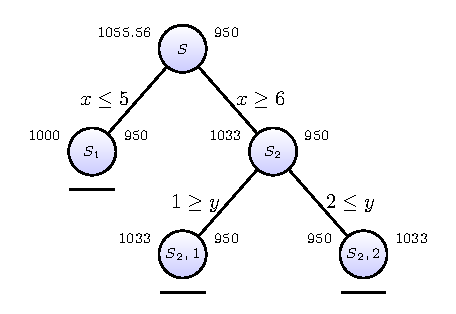
\includegraphics[scale = 0.5]{branch-and-bound}




Here is an example of branching on general integer variables.

\begin{example}{Branching on general integer variables}{}
%\textbf{Example: Branching on general integer variables}
Consider the two variable example with
 
 \begin{align*}
 \max & -3x_1 + 4x_2\\
 & 2x_1 + 2 x_2 \leq 13\\
 & -8 x_1 + 10x_2 \leq 41\\
 & 9x_1 + 5x_2 \leq 45\\
 & 0 \leq x_1 \leq 10, \text{ integer }\\
 & 0 \leq x_2 \leq 10, \text{ integer }
 \end{align*}
 
 
 
\tikzset{
  S/.style = {
    draw, rectangle, rounded corners=0.1cm,  
    top color=blue!10, bottom color=blue!10,
    %align=center,
    inner sep=5pt
  },
}

\tikzset{
  S/.style = {draw, rectangle, rounded corners=0.1cm, minimum size = 8mm,  top color=blue!10, bottom color=blue!10},% top color=white, bottom color=blue!20},
}




\tikzset{
  S/.style = {
    draw, rectangle, rounded corners=0.1cm,  
    top color=blue!10, bottom color=blue!10,
    align=center,
    inner sep=5pt
  },
}



\begin{tikzpicture}[-,thick]
\node[S, sibling distance=5cm, level distance=6.5cm, label={[blue]left:$t = 1$}, label = {above:\textbf{Root Node}}] 
{
    \begin{tabular}{c}
    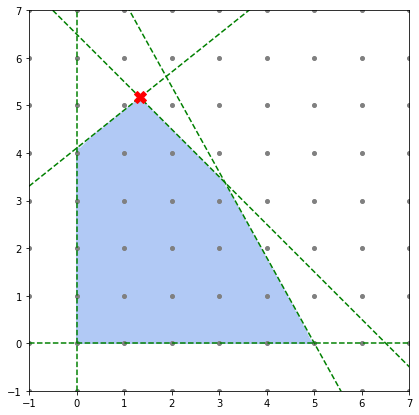
\includegraphics[scale=0.2]{branch-and-bound1} \\
    $x^* = (1.33, 5.167) $\\ $z^* = 16.664$\\ $ LB = -\infty$
    \end{tabular}
} 
[sibling distance=7cm, level distance=6.5cm]
%
child {node[S, label={[blue]left:$t = 2$}] 
    {
    \begin{tabular}{c}
    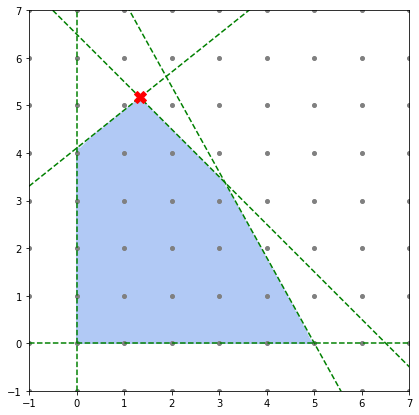
\includegraphics[scale=0.2]{branch-and-bound1} \\
    $x^* = (1, 4.9) $\\$z^* = 16.5998$\\$ LB = -\infty$
    \end{tabular}
    }
    [sibling distance=7cm, level distance=6.5cm]
    child {node[S, label={[blue]left:$t = 4$}, name=nodeInteger] 
        {
        \begin{tabular}{c}
        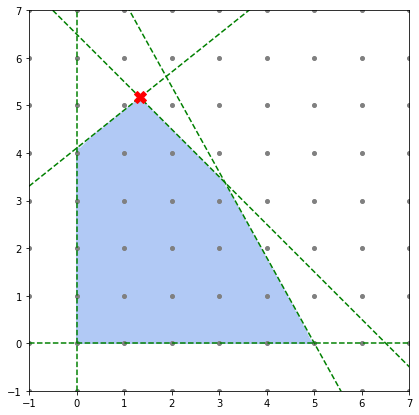
\includegraphics[scale=0.2]{branch-and-bound1} \\
        $x^* = (0,4)$\\$z^* = 16$\\$ LB = 16$
        \end{tabular}
        }
        edge from parent node[left] {$x_2 \leq 4$}
    }
    %
    child {node[S, label={[blue]right:$t =5$}, name=nodeInfeasible] 
        {
        \begin{tabular}{c}
        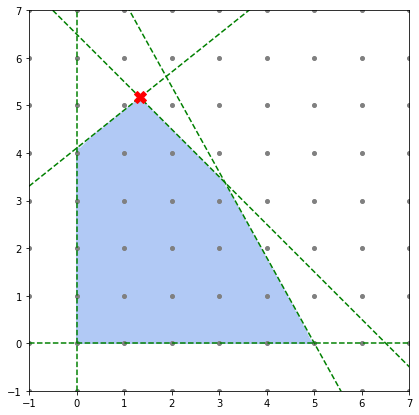
\includegraphics[scale=0.2]{branch-and-bound1} \\
        $x^* = \textrm{N/A}$\\$z^* = \textrm{N/A}$\\$ LB = \textrm{N/A}$
        \end{tabular}
        }
        edge from parent node[right] {$x_2 \geq 5$}
    }
%
edge from parent node[left] {$x_1 \leq 1$}
}
child {node[S, label={[blue]right:$t =3$}, name=nodeSuboptimal] 
    {
    \begin{tabular}{c}
    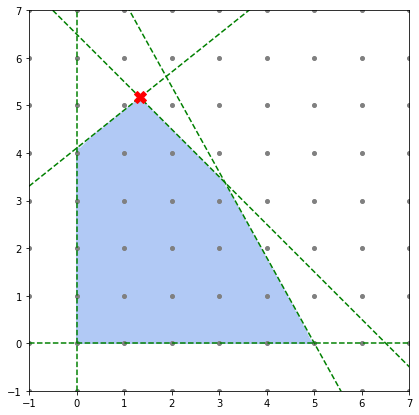
\includegraphics[scale=0.2]{branch-and-bound1} \\
    $x^* = (2, 4.5) $\\$z^* = 12.0$\\$ LB = -\infty$
    \end{tabular}
    }
    [sibling distance=5cm, level distance=2.8cm]
    edge from parent node[right] {$x_1 \geq 2$}
};

% Add the labels below the named nodes
\node[red, anchor=north, align=center] at (nodeInteger.south) {\rule{3cm}{0.8pt} \\ Integer};
\node[red, anchor=north, align=center] at (nodeInfeasible.south) {\rule{3cm}{0.8pt} \\ Infeasible};
\node[red, anchor=north, align=center] at (nodeSuboptimal.south) {\rule{3cm}{0.8pt} \\ Suboptimal};

\end{tikzpicture}
An optimal solution is concluded to be $x^* = (0,4)$ with objective value $z^* = 16$.
\end{example}

%
%
%$x =  [1.33, 5.167]$,   $\textrm{objective}  =  16.664$\\
%\noindent \includegraphicstatic[scale = 0.3]{branch-and-bound1}
%$x =  [1,  4.9]$,  $\textrm{objective} =  16.5998$\\
%$x =  [2,  4.5]$,  $\text{objective} =  12.0$\\
%\includegraphicstatic[scale = 0.3]{branch-and-bound2.png}
%
%Infeasible Region\\
%$x =  [0, 4]$,   $\text{objective} =  16.0$\\
%$x =  [2,  4.5]  \text{objective} =  12.0$\\
%\includegraphicstatic[scale = 0.3]{branch-and-bound3.png}
%
%This creates the following branch and bound tree.
%
%% Branch and bound tree for maximize knapsack
\tikzset{
  S/.style = {draw, rectangle, rounded corners=0.1cm, minimum size = 8mm,  top color=blue!10, bottom color=blue!10},% top color=white, bottom color=blue!20},
}
     \begin{tikzpicture}[-,thick]
\node[S,sibling distance=5cm, level distance=1.3cm, align=left, label={[blue]left:$t = 1$}, label = {above:\textbf{Root Node}}] 
	{$x^* = (1.33, 5.167) $\\ $z^* = 16.664$\\ $ LB = -\infty$} 
	[sibling distance=7cm, level distance=2.8cm,align=left]
	%
     	child {node[S, label={[blue]left:$t = 2$}] 
     		{$x^* = (1, 4.9) $\\$z^* = 16.5998$\\$ LB = -\infty$}
		[sibling distance=5cm, level distance=2.8cm,align=left]
		child {node[S, label={[blue]left:$t = 4$}, label = {[red]below: \rule{3cm}{0.8pt} \\ \centering Integer}] {$x^* = (0,4)$\\$z^* = 16$\\$ LB = 16$}
		%
     			edge from parent node[left] {$x_2 \leq 4$}}
			%
			child {node[S, label={[blue]right:$t =5$}, label = {[red]below: \rule{3cm}{0.8pt} \\ \centering Infeasible}] {$x^* = \textrm{N/A}$\\$z^* = \textrm{N/A}$\\$ LB = \textrm{N/A}$}[sibling distance=5cm, level distance=2.8cm,align=left]
			%
			edge from parent node[right] {$x_2 \geq 5$}
			}
%
   		edge from parent node[left] {$x_1 \leq 1$}
   }
     child {node[S, label={[blue]right:$t =3$},label = {[red]below: \rule{3cm}{0.8pt} \\ \centering Suboptimal}] 
     		{$x^* = (2, 4.5) $\\$z^* = 12.0$\\$ LB = -\infty$}
		[sibling distance=5cm, level distance=2.8cm,align=left]
		%
   		edge from parent node[right] {$x_1 \geq 2$}
   };

     \end{tikzpicture}


%\end{example}







%\begin{algorithm}[H]
%\caption{Branch and Bound for Binary Integer Program - Maximization}\label{alg:branch-and-bound-bip}
%\begin{algorithmic}[1]
%    \renewcommand{\algorithmicrequire}{\textbf{Input:}}
%    \renewcommand{\algorithmicensure}{\textbf{Output:}}
%    \algorithmicrequire Binary Integer Problem with max objective
%    \algorithmicensure Exact Optimal Solution \( x^* \)
%    \State Set \( LB = - \infty \).
%    \State Solve LP relaxation. 
%    \If{\( x^* \) is binary}
%        \State Stop!
%    \Else
%        \State Choose fractional entry \( x_i^* \).
%        \State Branch onto subproblems:
%        \Statex \hspace{2em} (i) \( x_i = 0 \)
%        \Statex \hspace{2em} (ii) \( x_i = 1 \)
%    \EndIf
%    \State Solve LP relaxation of any subproblem.
%    \If{LP relaxation is infeasible}
%        \State Prune this node as \textbf{"Infeasible"}
%    \ElsIf{\( z^* < LB \)}
%        \State Prune this node as \textbf{"Suboptimal"}
%    \ElsIf{\( x^* \) is binary}
%        \State Prune this node as \textbf{"Binary"}
%        \State Update \( LB = \max(LB, z^*) \).
%    \Else
%        \State Choose fractional entry \( x_i^* \).
%        \State Branch onto subproblems:
%        \Statex \hspace{2em} (i) \( x_i = 0 \)
%        \Statex \hspace{2em} (ii) \( x_i = 1 \)
%        \State Return to step 2 until all subproblems are pruned.
%    \EndIf
%    \State Return best binary solution found.
%\end{algorithmic}
%\end{algorithm}

%
%\subsection{Knapsack Problem  and 0/1 branching}
%
%Consider the problem 
%
%\begin{align*}
%\max \quad & 16x_1 + 22x_2 + 12x_3 + 8 x_4\\
%\st & 5x_1 + 7x_2 + 4x_3 + 3x_4 \leq 14\\
%& 0 \leq x_i \leq 1 \ \ i=1,2,3,4\\
%& x_i \in \{0,1\} \ \ i=1,2,3,4
%\end{align*}
%
%\textbf{Question: What is the optimal solution if we remove the binary constraints?}




%\begin{align*}
%\max \quad & c_1 x_1 + c_2 x_2 + c_3 x_3 + c_4 x_4\\
%\st & a_1 x_1 + a_2 x_2 + a_3 x_3 + a_4 x_4 \leq b\\
%& 0 \leq x_i \leq 1 \ \ i=1,2,3,4\\
%\end{align*}
%
%\textbf{Question: How do I find the solution to this problem?}
%
%
%\begin{align*}
%\max \quad & c_1 x_1 + c_2 x_2 + c_3 x_3 + c_4 x_4\\
%\st & (a_1 - A)x_1 + (a_2-A) x_2 + (a_3-A) x_3 + (a_4-A) x_4 \leq 0\\
%& 0 \leq x_i \leq m_i \ \ i=1,2,3,4\\
%\end{align*}

%\textbf{Question: How do I find the solution to this problem?}
%
%
%
%Consider the problem 
%
%\begin{align*}
%\max \quad & 16x_1 + 22x_2 + 12x_3 + 8 x_4\\
%\st & 5x_1 + 7x_2 + 4x_3 + 3x_4 \leq 14\\
%& 0 \leq x_i \leq 1 \ \ i=1,2,3,4\\
%& x_i \in \{0,1\} \ \ i=1,2,3,4
%\end{align*}
%
%We can solve this problem with branch and bound.
%
%
%The optimal solution was found at $t=5$ at subproblem 6 to be $x^* = (0,1,1,1)$, $z^* = 42$.
%
%





\section{Cutting Planes}
Cutting planes are additional inequalities that are valid for the feasible integer solutions that  cut off part of the LP relaxation.  Cutting planes can create a tighter description of the feasible region that allows for the optimal solution to be obtained by simply solving a strengthened linear relaxation. 

We begin with an example of problem specific inequalites that apply only to certain structured constraints.

\subsection{Cover Inequalities}
Consider the binary knapsack problem
\begin{align*}
\max \ \ & x_1 + 2x_2 + x_3 + 7 x_4\\
\text{s.t.} \ \ & 100 x_1 + 70x_2 + 50 x_3 + 60 x_4 \leq 150\\
& x_i  \text{ binary  for } i =1, \dots, 4
\end{align*}

A \emph{cover} $S$ is any subset of the variables whose sum of weights exceed the capacity of the right hand side of the inequality.\\
For example, $S = \{1,2,3,4\}$ is a cover since $100 + 70 + 50 + 60 > 150$.\\
Since not all variables in the cover $S$ can be in the knapsack simultaneously, we can enforce the \emph{cover inequality}
\begin{equation}
\sum_{i \in S} x_i \leq |S| - 1 \ \ \ \Rightarrow \ \ \ \ x_1 + x_2 + x_3 + x_4 \leq 4 - 1 = 3.
\end{equation}
Note, however, that there are other covers that use fewer variables.\\

A \emph{minimal cover} is a subset of variables such that no other subset of those variables is also a cover.  For example, consider the cover $S' = \{1,2\}$.  This is a cover since $100 + 70 > 150$.  Since $S'$ is a subset of $S$, the cover $S$ is not a minimal cover.  In fact, $S'$ is a minimal cover since there are no smaller subsets of the set $S'$ that also produce a cover.
In this case, we call the corresponding inequality a \emph{minimal cover inequality}.  That is, the inequality
\begin{equation}
x_1 + x_2 \leq 2 - 1 = 1
\end{equation}
is a minimal cover inequality for this problem.   The minimal cover inequalities are the "strongest" of all cover inequalities.

\emph{Find the two other minimal covers (one of size 2 and one of size 3) and write their corresponding minimal cover inequalities.}

\begin{solution}{}{}{}
The other minimal covers are 
\begin{equation}
S = \{1,4\} \ \ \Rightarrow \ \ \ x_1 + x_4 \leq 1
\end{equation}
and
\begin{equation}
S = \{2,3,4\} \ \ \Rightarrow \ \ \ x_2 + x_3 + x_4 \leq 2
\end{equation}
\end{solution}





\subsection{Chv\'atal Cuts}


Chv\'atal Cuts are a general technique to produce new inequalities that are valid for feasible integer points.  


\begin{general}{Chv\'atal Cuts}{}
Suppose 
\begin{equation}
a_1 x_1 + \dots + a_n x_n \leq d
\end{equation}
is a valid inequality for the polyhedron $P = \{ x \in \R^n : Ax \leq b, x \geq 0\}$, then 
\begin{equation}
\label{eq:chvatal}
\lfloor a_1\rfloor x_1 + \dots + \lfloor a_n\rfloor  x_n \leq \lfloor d\rfloor
\end{equation}
is valid for the integer points in $P$, that is, it is valid for the set $P \cap \Z^n$.  Equation~\eqref{eq:chvatal} is called a Chv\'atal Cut.
\end{general}


We will illustrate this idea with an example.


\begin{example}{}{}
Recall example~\ref{ex:min-coins}.  The model was\\
\textbf{Model}
\begin{align*}
\min \quad & p + n + d + q & \text{ total number of coins used}\\
\text{ s.t. } \quad & p + 5n + 10d + 25 q = 83 & \text{sums to } 83 \cent\\
& p,d,n,q \in \Z_+ & \text{each is a non-negative integer}
\end{align*}

From the equality constraint we can derive several inequalities.
\begin{enumerate}
\item Divide by 25 and round down both sides:
\[
\frac{p + 5n + 10d + 25 q}{25} = 83/25 \quad \Rightarrow \quad q \leq 3 
\]
\item Divide by 10 and round down both sides:
\[
\frac{p + 5n + 10d + 25 q}{10} = 83/10 \quad \Rightarrow \quad d + 2q \leq 8 
\]
\item Divide by 5 and round down both sides:
\[
\frac{p + 5n + 10d + 25 q}{10} = 83/5 \quad \Rightarrow \quad n + 2d  + 5q \leq 16
\]
\item Multiply by 0.12 and round down both sides:
\[
0.12(p + 5n + 10d + 25 q = 0.12 (83) \quad \Rightarrow \quad d  + 3q \leq 9
\]
\end{enumerate}
These new inequalities are all valid for the integer solutions.  Consider the new model:\\

\textbf{New Model}
\begin{align*}
\min \quad & p + n + d + q & \text{ total number of coins used}\\
\text{ s.t. } \quad & p + 5n + 10d + 25 q = 83 & \text{sums to } 83 \cent\\
& q \leq 3\\
& d + 2q \leq 8 \\
& n + 2d  + 5q \leq 16\\
& d  + 3q \leq 9\\
& p,d,n,q \in \Z_+ & \text{each is a non-negative integer}
\end{align*}

The solution to the LP relaxation is exactly $q = 3, d = 0, n = 1, p = 3$, which is an integral feasible solution, and hence it is an optimal solution.
\end{example}

\subsection{Cutting Planes Procedure}
Cutting planes can be constructed dynamically so that we only look for cuts that are critical to proving optimality of the problem.

This is done by iteratively solving a relaxation, adding a cut to improve the relaxation, and then resolving the relaxation.   

Here is the basic algorithm.
\begin{algorithm}
\caption{(Pure) Cutting Plane Procedure}
\label{alg:cutting-plane-procedure}
\begin{algorithmic}[1]
    \State \textbf{Input:} Current LP relaxation.
    \State \textbf{Output:} Integral solution (if exists).
    
    \Procedure{CuttingPlane}{}
        \While{True}
            \State Solve the current LP relaxation.
            \If{solution is integral}
                \State \Return that solution.
                \State \textbf{STOP}
            \EndIf
            \State Add a cutting plane (or many cutting planes) that cut off the LP-optimal solution.
        \EndWhile
    \EndProcedure
\end{algorithmic}
\end{algorithm}

Refer to the cutting plane procedure in Figure~\ref{alg:cutting-plane-procedure}.

\begin{figure}[H]
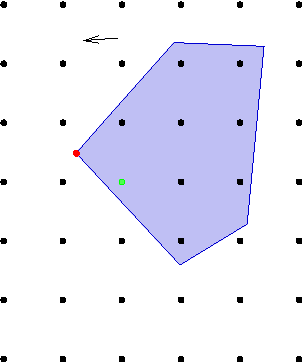
\includegraphics[scale = 0.4]{optimization/figures/figures-static/figureCutttingPlane1.pdf} 
\hspace{0.3cm}
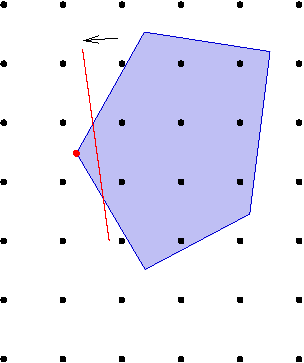
\includegraphics[scale = 0.4]{optimization/figures/figures-static/figureCutttingPlane2}
\hspace{0.3cm}
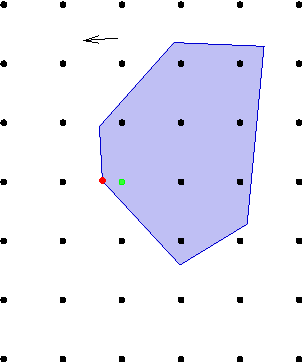
\includegraphics[scale = 0.4]{optimization/figures/figures-static/figureCutttingPlane3}
\hspace{0.3cm}
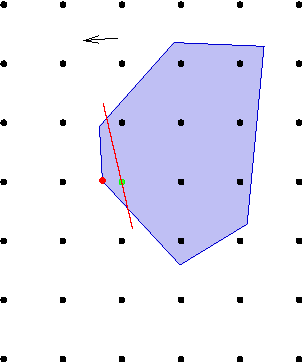
\includegraphics[scale = 0.4]{optimization/figures/figures-static/figureCutttingPlane4}
\hspace{0.3cm}
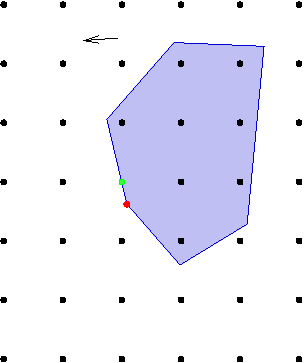
\includegraphics[scale = 0.4]{optimization/figures/figures-static/figureCutttingPlane5}
\hspace{0.3cm}
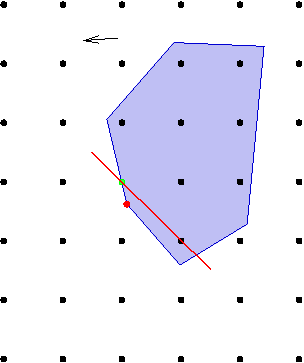
\includegraphics[scale = 0.4]{optimization/figures/figures-static/figureCutttingPlane6}
\vspace{0.3cm}
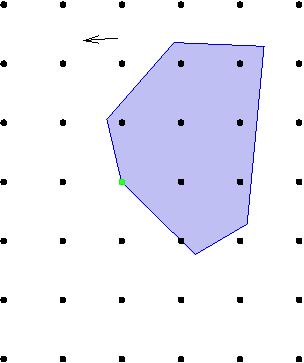
\includegraphics[scale = 0.4]{optimization/figures/figures-static/figureCutttingPlane7}
\caption{The cutting plane procedure.}
\label{fig:cutting-plane-procudure}
\end{figure}

In practice, this procedure is integrated in some with with branch and bound and also other primal heuristics.

%\begin{table}
%\centering\begin{tabular}{|>{\centering\arraybackslash}m{3cm}|>{\centering\arraybackslash}m{5cm}|} \hline\textbf{Topic} & \textbf{Paragraph} \\\hline \hlineTopic 1 & This is a paragraph. This is a paragraph. This is a paragraph.\\\hline\end{tabular}
%\end{table}

Here is a concrete example of how this could play out.

\begin{table}[H]
\centering\begin{tabular}{>{\centering\arraybackslash}m{5cm}>{\centering\arraybackslash}m{10cm}}
 \hline
\textbf{Model} & \textbf{LP Solution} \\\hline \hline

$$
\begin{array}{lrl}
\max \ & x_1 + x_2\\
\text{subject to  } &  -2x_1 + x_2 &\leq 0.5\\
& x_1 + 2x_2 &\leq 10.5\\
& x_1 - x_2 &\leq 0.5\\
& - 2x_1 - x_2 &\leq -2
\end{array} 
$$
&
\includegraphicstatic[scale = 0.5]{cutting-plane-1-picture}\\
$$
\begin{array}{lrl}
\max \ & x_1 + x_2\\
\text{subject to  } &  -2x_1 + x_2 &\leq 0.5\\
& x_1 + 2x_2 &\leq 10.5\\
& x_1 - x_2 &\leq 0.5\\
& - 2x_1 - x_2 &\leq -2\\
& \tred{x_1} &\tred{\leq 3}
\end{array} 
$$
&
\includegraphicstatic[scale = 0.5]{cutting-plane-2-picture}\\
$$
\begin{array}{lrl}
\max \ & x_1 + x_2\\
\text{subject to  } &  -2x_1 + x_2 &\leq 0.5\\
& x_1 + 2x_2 &\leq 10.5\\
& x_1 - x_2 &\leq 0.5\\
& - 2x_1 - x_2 &\leq -2\\
& \tred{x_1} & \tred{\leq 3}\\
& \tred{x_1 + x_2} & \tred{\leq 6}
\end{array} 
$$
&
\includegraphicstatic[scale = 0.5]{cutting-plane-3-picture}\\
\hline
 \end{tabular}
\end{table}
\subsection{Gomory Cuts}
Gomory cuts are a type of Chv\'atal cut that is derived from the simplex tableau and can be generated dynamically, and thus is a viable candidate to implement the cutting plane procedure.

Specifically, suppose that 
\begin{equation}
\label{eq:tableau-row}
 x_j + \sum_{i\in N} \tilde a_i x_i = \tilde b_j
\end{equation}
is an equation in the optimal simplex tableau. 

\begin{general}{Gomory Cut}{}
The Gomory cut corresponding to the tableau row ~\eqref{eq:tableau-row} is

\begin{equation}
\label{eq:gomory-cut}
\sum_{i\in N} (\tilde a_i - \lfloor \tilde a_i \rfloor) x_i \geq \tilde b_j - \lfloor \tilde b_j\rfloor
\end{equation}


\end{general}


We will solve the following problem using only Gomory Cuts.
\begin{equation*}
\begin{array}{lrcl}
\min & x_1 - 2x_2\\
\st & -4x_1 + 6x_2  & \leq & 9\\
& x_1 + x_2   & \leq & 4\\
& x \geq 0 & , & x_1,x_2 \in \Z
\end{array}
\end{equation*}

\textbf{Step 1:} The first thing to do is to put this into standard from by appending slack variables.
\begin{equation}
\label{eq:gomory-standard-form}
\begin{array}{lrcl}
\min & x_1 - 2x_2\\
\st & -4x_1 + 6x_2 + s_1 & = & 9\\
& x_1 + x_2 + s_2  & = & 4\\
& x \geq 0 & , & x_1,x_2 \in \Z
\end{array}
\end{equation}

We can apply the simplex method to solve the LP relaxation.\\
\begin{tabular}{cc}
Initial Basis & 
%\begin{center}
\begin{tabular}{|lr|rrrr|}
\hline
 Basis & RHS & $x_1$ & $x_2$ & $s_1$ & $s_2$ \\
 \hline
 $z$     & 0.0 & 1.0   & -2.0  & 0.0   & 0.0   \\
 \hline
 $s_1$ & 9.0 & -4.0  & 6.0   & 1.0   & 0.0   \\
 $s_2$ & 4.0 & 1.0   & 1.0   & 0.0   & 1.0   \\
\hline
\end{tabular}\\
%\end{center}\\
\vdots & \vdots  \\
Optimal Basis & 
%Pivoting to the optimal basis, we have
%\begin{center}
\begin{tabular}{|lr|rrrr|}
\hline
 Basis & RHS  & $x_1$ & $x_2$ & $s_1$ & $s_2$ \\
 \hline
 $z$     & -3.5 & 0.0   & 0.0   & 0.3   & 0.2   \\
 \hline
 $x_1$ & 1.5  & 1.0   & 0.0   & -0.1  & 0.6   \\
 $x_2$ & 2.5  & 0.0   & 1.0   & 0.1   & 0.4   \\
\hline
\end{tabular}
%\end{center}
\end{tabular}

This LP relaxation produces the fractional basic solution $x_{LP} = (1.5, 2.5)$.


\begin{example}{}{}\textbf{(Gomory cut  removes LP solution)}{}
 We now identify an integer variable $x_i$ that has a fractional basic solution.  Since both variables have fractional values, we can choose either row to make a cut.  Let's focus on the row corresponding to $x_1$.

The row from the tableau expresses the equation 
\begin{equation}
x_1 - 0.1 s_1 + -0.6 s_2 = 1.5.
\end{equation}

Applying the Gomory Cut~\eqref{eq:gomory-cut}, we have the inequality 
\begin{equation}
\label{eq:gomory-cut-ex1}
0.9 s_1 + 0.4 s_2 \geq 0.5.
\end{equation}

The current LP solution is $(x_{LP}, s_{LP}) = (1.5, 2.5,0,0)$.  Trivially, since $s_1, s_2 = 0$, the inequality is violated.
\end{example}

\begin{example}{\textbf{(Gomory Cut in Original Space)}}{}

The Gomory Cut~\eqref{eq:gomory-cut-ex1} can be rewritten in the original variables using the equations from~\eqref{eq:gomory-standard-form}.  That is, we can use the equations
\begin{equation}
\label{eq:gomory-standard-form-equations}
\begin{array}{lrcl}
 & s_1 & = & 9 + 4x_1 - 6x_2\\
&s_2  & = & 4 - x_1 - x_2,
\end{array}
\end{equation}
which transforms the Gomory cut into the original variables to create the inequality
\begin{equation*}
\label{eq:gomory-cut-ex1-original}
0.9 (9 + 4x_1 - 6x_2) + 0.4(4 - x_1 - x_2) \geq 0.5.
\end{equation*}
or equivalently
\begin{equation}
\label{eq:gomory-cut-ex1-original}
- 3.2 x_1 + 5.8 x_2 \leq 9.2.
\end{equation}
%\textbf{Check!} We can now check if this inequality cuts off the current LP optimal solution.
%To see this, let's plug in $(x_{LP}, s_{LP}) = (1.5, 2.5,0,0)$.
%
%\begin{equation}
%\label{eq:gomory-cut-ex1-original}
%- 3.2 x_1 + 5.8 x_2 = - 3.2 (1.5) + 5.8 (2.5) = 9.7 > 9.2
%\end{equation}
%Thus, this LP solution is violated by the new Gomory Cut.

As you can see, this inequality does cut off the current LP relaxation.
%\includegraphics[scale = 0.5]{this-graphic.}

\end{example}


\begin{example}{\textbf{(Gomory  cuts plus new tableau)}}{}
Now we add the slack variable $s_3 \geq 0$ to make the equation
\begin{equation}
0.9 s_1 + 0.4 s_2 - s_3 = 0.5.
\end{equation}


\end{example}


Next, we need to solve the new linear programming relaxation and continue the cutting plane procedure.




\section{Interpreting Output Information and Progress}
\todoSection{Write this section.  Include screenshot of a solver log}


\includefigurestatic[This shows the progress of the solver over time.][width=0.90\linewidth][h]{solve_progress1.png}

\includefigurestatic[This shows the progress of the solver over time.][width=0.90\linewidth][h]{solve_progress2.png}

\section{Branching Decision Rules in Integer Programming}
\begin{outcome}
A thorough study of branching decision rults is not necessary at this point, but we add some high level discussion here to demonstrate that this is an important part of solving integer programs effeciently.
\end{outcome}

Integer programming (IP) is a mathematical optimization technique where some or all of the variables are restricted to take integer values. One of the most popular methods for solving integer programming problems is the branch-and-bound method. Central to the branch-and-bound method is the concept of branching, where the solution space is recursively divided into smaller subproblems. The decision on how and where to branch is governed by branching decision rules.

\paragraph{Importance of Branching Rules}

The efficiency of the branch-and-bound method heavily depends on the choice of branching rules. A good branching rule can significantly reduce the number of subproblems that need to be explored, leading to faster solution times. Conversely, a poor branching rule can lead to an exponential increase in the number of subproblems, making the problem intractable.

\paragraph{Common Branching Rules}

There are several branching rules that have been proposed in the literature. Some of the most common ones include:

\begin{itemize}
    \item \textbf{Most Fractional Variable Rule:} This rule selects the variable that has the fractional part closest to 0.5 for branching. The rationale is that this variable is the most uncertain in terms of its integer value.
    
    \item \textbf{Least Fractional Variable Rule:} Contrary to the most fractional variable rule, this rule selects the variable with the fractional part furthest from 0.5.
    
    \item \textbf{Strong Branching:} This rule evaluates the impact of branching on a few variables and selects the one that seems most promising in terms of reducing the objective function value.
    
    \item \textbf{Pseudocost Branching:} Pseudocosts estimate the impact of branching on a particular variable based on historical data from previous branchings on that variable. For each variable, two pseudocosts are maintained: one for the upward branch (rounding up) and one for the downward branch (rounding down). The variable with the highest expected improvement in the objective function, based on its pseudocosts, is selected for branching.
\end{itemize}
\paragraph{Problem specific branching}
Reformulating integer programming problems can reveal hidden structures beneficial for branching. For instance, transforming a problem or linearizing constraints might introduce new variables that offer insightful branching points. These auxiliary variables, emerging from reformulations like the cutting plane method, often encapsulate the problem's combinatorial essence. Branching on them can lead to tighter bounds or more effective pruning of infeasible regions.

While traditional branching is binary, considering multi-way branching—where a node splits into more than two branches—can be advantageous for problems where variables have multiple discrete values. This approach allows for simultaneous exploration of several potential solution paths, enhancing the efficiency of the search process.

In essence, delving into a problem's specific structure and reformulations can pave the way for innovative and more efficient branching strategies.


\paragraph{Advanced Branching Techniques with Machine Learning}

Branching algorithms in commercial solvers are highly tuned for performance. They often incorporate advanced strategies, including periodic restarts, to improve the branching tree's structure and efficiency. In recent years, machine learning techniques have been employed and studied to devise better branching rules. These techniques can be tailored for specific problem classes or designed for general use cases. Machine learning can be applied in an offline setting, where the algorithm learns from a set of instances and then applies the knowledge to new instances, or in an online fashion, where the algorithm refines its branching rules during the branching process. Furthermore, machine learning has been utilized to estimate the overall size of the branch-and-bound tree required to reach optimality. Notably, such techniques have been implemented in the open-source solver SCIP.


The choice of branching rule is crucial in determining the efficiency of the branch-and-bound algorithm for integer programming. With the advent of machine learning and continuous advancements in optimization techniques, the landscape of branching strategies is rapidly evolving, offering promising avenues for even more efficient integer programming solutions.


There is a few clever ideas out there on how to choose which variables to branch on.  We will not go into this here.  But for the interested reader, look into 
\begin{itemize}
\item Strong Branching
\item Pseudo-cost Branching
\end{itemize}

\section{Decomposition Methods - Advanced approaches to integer programming}
\begin{outcome}
A thorough study of the decompsition approaches discussed in this section are not necessary at this point, but we add some high level discussion here regarding the techniques to give the reader a sense of what approaches can be taken when the models chosen are not solving fast enough.  
\end{outcome}


We will discuss briefly three key decomposition approaches: Lagrangian Relaxation, Dantzig-Wolfe Reformulation (with column generation and branch and price), and Benders Decomposition.

We will give more attention to these approaches in a much later part of this book on Advanced Integer Programming Techniques.

\subsection{Lagrangian Relaxation}



Lagrangian relaxation is a powerful technique in integer programming designed to simplify complex problems by moving certain complicating constraints into the objective function. The essence of this method lies in "relaxing" these constraints, allowing them to be violated at a cost. This is achieved by associating each relaxed constraint with a Lagrange multiplier, which then penalizes the objective function based on the degree of violation.

The primary advantage of Lagrangian relaxation is the creation of a strong relaxation for the problem. By transforming the original problem into a more tractable one, solutions can be obtained more efficiently, often providing good bounds for the original problem. Moreover, the dual values of the Lagrange multipliers can offer insights into the relative importance of the relaxed constraints, guiding further refinements or heuristic approaches.

Within a branch-and-bound framework, Lagrangian relaxation can be particularly effective. At each node of the branching tree, the Lagrangian relaxation can be solved to obtain bounds for the subproblem. If the bound indicates that the node cannot lead to a better solution than the current best-known one, the node can be pruned, reducing the overall search space. Additionally, solutions to the relaxed problem can guide branching decisions or serve as starting solutions for heuristics, accelerating the overall solution process.

In summary, Lagrangian relaxation offers a strategic approach to handle complicating constraints in integer programming, facilitating the generation of strong relaxations and enhancing the efficiency of algorithms like branch-and-bound.



See~\cite{Fisher2004}  \href{https://my.eng.utah.edu/~kalla/phy_des/lagrange-relax-tutorial-fisher.pdf}{(link)} for a tutorial on Lagrangian Relaxations.


\subsection{Dantzig-Wolfe Reformulation and Column Generation}

Dantzig-Wolfe reformulation is a technique in mathematical optimization that decomposes a problem into subproblems by exploiting its block structure. Specifically, it's applied to problems where the constraints can be divided into groups that interact only through certain linking constraints. The reformulation expresses the original variables as combinations of new variables, often referred to as "columns," which represent feasible solutions to the subproblems.

The primary advantage of Dantzig-Wolfe reformulation is that it transforms the original problem into a master problem with a potentially much-reduced set of variables (columns). However, the challenge is that the number of potential columns can be exponentially large, making it impractical to enumerate them all. This is where column generation comes into play.

\paragraph{Column Generation} is an iterative method to handle the large set of potential columns. Instead of considering all columns simultaneously, the algorithm starts with a subset of promising columns. The master problem is solved with this subset, and then a pricing subproblem is tackled to identify if there are any columns (feasible solutions to the subproblems) that can improve the master problem's objective. If such columns are found, they are added to the master problem, and the process repeats. This "generate-and-solve" approach continues until no more beneficial columns can be identified.

\paragraph{Branch-and-Price} is an extension of the branch-and-bound method that incorporates column generation. In a branch-and-price algorithm, the branching process is applied to the master problem, but at each node of the branching tree, column generation is used to dynamically generate the necessary columns. This approach combines the power of Dantzig-Wolfe reformulation and column generation with the systematic search of branch-and-bound, allowing for the efficient solution of large-scale integer programming problems with a decomposable structure.

In summary, Dantzig-Wolfe reformulation provides a foundation for decomposing complex optimization problems. When combined with column generation and the branch-and-price framework, it offers a potent toolkit for tackling large-scale, structured integer programming challenges.


Dantzig-Wolfe reformulation, combined with column generation and branch-and-price techniques, has been instrumental in solving a variety of large-scale combinatorial optimization problems. Some of the key applications include:

\begin{enumerate}
    \item \textbf{Cutting Stock Problem:} Perhaps one of the most classic applications, the cutting stock problem involves determining the optimal way to cut raw materials (like rolls of paper or metal beams) to meet specific demand requirements while minimizing waste. The columns in this context represent different cutting patterns.
    
    \item \textbf{Vehicle Routing Problem (VRP):} In the VRP, a fleet of vehicles must deliver goods to a set of customers in the most efficient manner. The challenge is to determine routes for each vehicle such that all customers are served, and the total routing cost is minimized. Columns can represent feasible routes or segments of routes for the vehicles.
    
    \item \textbf{Crew Scheduling:} Airlines and railways face the challenge of assigning crew members to flights or trains while adhering to regulations and minimizing costs. In this context, columns can represent feasible schedules or rotations for the crew members.
    
    \item \textbf{Set Partitioning and Covering Problems:} These problems arise in various applications, such as airline crew scheduling, school timetabling, and frequency assignment in telecommunications. Columns represent subsets of items or tasks that can be grouped or covered together.
    
    \item \textbf{Capacitated Arc Routing Problem:} Similar to the VRP, but the focus is on serving demands located on edges (or arcs) of a network, like snow plowing or garbage collection on street networks. Columns can represent feasible routes on the network.
    
    \item \textbf{Bin Packing:} This problem involves packing items of different volumes into a finite number of bins in a way that minimizes the number of bins used. Columns represent feasible packing patterns for the bins.
\end{enumerate}

These applications underscore the versatility and power of Dantzig-Wolfe reformulation and associated techniques. By decomposing complex problems into more manageable subproblems, these methods provide a structured and efficient approach to tackle large-scale, real-world optimization challenges.



\subsection{Benders Decomposition}

Benders' decomposition is a mathematical optimization technique designed to tackle problems with a specific structure, where decision variables can be partitioned into two sets, often referred to as the "master" and "subproblem" variables. The primary idea behind Benders' decomposition is to solve the problem iteratively, addressing the master problem and subproblem separately, and then linking them through optimality and feasibility cuts.

The method begins by solving a simplified version of the master problem without considering the complicating constraints associated with the subproblem. Once a solution is obtained, it's used to generate and solve the subproblem. The outcome of the subproblem then informs whether the current master solution is feasible or not. If infeasible, a feasibility cut is added to the master problem. If feasible but suboptimal, an optimality cut is introduced. This iterative process continues until convergence is achieved.

One of the most notable applications of Benders' decomposition is in Stochastic Programming. Stochastic Programming deals with optimization problems where some parameters are uncertain and described by probability distributions. In such problems, the decision-making process is often split into two stages: "here-and-now" decisions made before the realization of uncertainty and "wait-and-see" decisions made after. Benders' decomposition is particularly useful here, as the master problem can handle the "here-and-now" decisions, while the subproblem manages the "wait-and-see" decisions for various scenarios of uncertainty. This decomposition allows for efficient exploration of the solution space and provides a structured way to handle the complexities introduced by uncertainty.

In summary, Benders' decomposition offers a strategic approach to decompose and solve complex optimization problems, with its application in Stochastic Programming standing out as a testament to its efficacy in handling uncertainty and multi-stage decision-making.


\section{Literature and Resources}


\begin{resource}
LP Rounding
\begin{itemize}
\item  \href{https://youtu.be/Az7HUuq4SOI?t=189}{Video! - Michel Belaire (EPFL) looking at rounding the LP solution to an IP solution}
\end{itemize}

Fractional Knapsack problem
\begin{itemize}
\item \href{https://youtu.be/m1p-eWxrt6g}{Video solving the Fractional Knapsack Problem}
\item \href{https://www.geeksforgeeks.org/fractional-knapsack-problem/}{Blog solving the Fractional Knapsack Problem}
\end{itemize}

Branch and Bound
\begin{itemize}
\item \href{https://www.youtube.com/watch?v=SdXPNaID-T8}{Video! -  Michel Belaire (EPFL) Teaching Branch and Bound Theory}
\item \href{https://www.youtube.com/watch?v=nKXZYQUtvAY}{Video! -  Michel Belaire (EPFL) Teaching Branch and Bound with Example}
\item See \href{http://web.tecnico.ulisboa.pt/mcasquilho/compute/_linpro/TaylorB_module_c.pdf}{Module by Miguel Casquilho} for some nice notes on branch and bound.
\end{itemize}

Gomory Cuts
\begin{itemize}
\item \href{https://www.youtube.com/watch?v=1i0rKtH_YPs&list=PLNMgVqt8MREx6Nex1Q9003vrZem-JXNvX&index=28&ab_channel=EducationalDocumentaries}{Pascal Van Hyndryk (Georgia Tech) Teaching Gomory Cuts}
\item \href{https://www.youtube.com/watch?v=VdXHGNDnjjo}{Michel Bierlaire (EPFL) Teaching Gomory Cuts}
\end{itemize}

Benders Decomposition
\begin{itemize}
\item \href{https://www.juliaopt.org/notebooks/Shuvomoy%20-%20Benders%20decomposition.html}{Benders Decomposition - Julia Opt}
\item \href{https://www.youtube.com/watch?v=8vUNXHwVnC8}{Youtube!  SCIP lecture}
\end{itemize}
\end{resource}


%\end{document}
